%%%%%%%%%%%%%%%%%%%%%%%%%%%%%%%%%%%%%%%%%%%%%%%%%%%%%%%%%%%%%%%%%%%%%%%%%%%%%%%%
% Version Control Systems
%
% Author: FOSSEE 
% Copyright (c) 2009, FOSSEE, IIT Bombay
%%%%%%%%%%%%%%%%%%%%%%%%%%%%%%%%%%%%%%%%%%%%%%%%%%%%%%%%%%%%%%%%%%%%%%%%%%%%%%%%

\documentclass[14pt,compress]{beamer}

\mode<presentation>
{
  \usetheme{Warsaw}
  \useoutertheme{infolines}
  \setbeamercovered{transparent}
}

\usepackage[english]{babel}
\usepackage[latin1]{inputenc}
%\usepackage{times}
\usepackage[T1]{fontenc}

% Taken from Fernando's slides.
\usepackage{ae,aecompl}
\usepackage{mathpazo,courier,euler}
\usepackage[scaled=.95]{helvet}

\definecolor{darkgreen}{rgb}{0,0.5,0}

\usepackage{listings}
\lstset{language=Python,
    basicstyle=\ttfamily\bfseries,
    commentstyle=\color{red}\itshape,
  stringstyle=\color{darkgreen},
  showstringspaces=false,
  keywordstyle=\color{blue}\bfseries}

%%%%%%%%%%%%%%%%%%%%%%%%%%%%%%%%%%%%%%%%%%%%%%%%%%%%%%%%%%%%%%%%%%%%%%
% Macros
\setbeamercolor{emphbar}{bg=blue!20, fg=black}
\newcommand{\emphbar}[1]
{\begin{beamercolorbox}[rounded=true]{emphbar} 
      {#1}
 \end{beamercolorbox}
}
\newcounter{time}
\setcounter{time}{0}
\newcommand{\inctime}[1]{\addtocounter{time}{#1}{\tiny \thetime\ m}}

\newcommand{\typ}[1]{\lstinline{#1}}

\newcommand{\kwrd}[1]{ \texttt{\textbf{\color{blue}{#1}}}  }

%%% This is from Fernando's setup.
% \usepackage{color}
% \definecolor{orange}{cmyk}{0,0.4,0.8,0.2}
% % Use and configure listings package for nicely formatted code
% \usepackage{listings}
% \lstset{
%    language=Python,
%    basicstyle=\small\ttfamily,
%    commentstyle=\ttfamily\color{blue},
%    stringstyle=\ttfamily\color{orange},
%    showstringspaces=false,
%    breaklines=true,
%    postbreak = \space\dots
% }

%%%%%%%%%%%%%%%%%%%%%%%%%%%%%%%%%%%%%%%%%%%%%%%%%%%%%%%%%%%%%%%%%%%%%%
% Title page
\title[Version Control Systems]{SEES: Version Control Systems}

\author[FOSSEE] {FOSSEE}

\institute[IIT Bombay] {Department of Aerospace Engineering\\IIT Bombay}
\date[]{}
%%%%%%%%%%%%%%%%%%%%%%%%%%%%%%%%%%%%%%%%%%%%%%%%%%%%%%%%%%%%%%%%%%%%%%

%\pgfdeclareimage[height=0.75cm]{iitmlogo}{iitmlogo}
%\logo{\pgfuseimage{iitmlogo}}


%% Delete this, if you do not want the table of contents to pop up at
%% the beginning of each subsection:
\AtBeginSubsection[]
{
  \begin{frame}<beamer>
    \frametitle{Outline}
    \tableofcontents[currentsection,currentsubsection]
  \end{frame}
}

\AtBeginSection[]
{
  \begin{frame}<beamer>
    \frametitle{Outline}
    \tableofcontents[currentsection,currentsubsection]
  \end{frame}
}

% If you wish to uncover everything in a step-wise fashion, uncomment
% the following command: 
%\beamerdefaultoverlayspecification{<+->}

%%\includeonlyframes{current,current1,current2,current3,current4,current5,current6}

%%%%%%%%%%%%%%%%%%%%%%%%%%%%%%%%%%%%%%%%%%%%%%%%%%%%%%%%%%%%%%%%%%%%%%
% DOCUMENT STARTS
\begin{document}

\begin{frame}
  \maketitle
\end{frame}

% CREATING TOC 
\begin{frame}
  \frametitle{Outline}
  \tableofcontents
  % You might wish to add the option [pausesections]
\end{frame}

%% There are some %$ used just to minimise the effect of $ sign used in lstlisting. In emacs it looks unhealthy.

% Introduction to course-need of version control, history, options available.
\section{Introduction}

\begin{frame}
  \frametitle{What is Version Control?}
  \begin{block}{From a blog post}
    ``Version control (or source control) is nothing more arcane than keeping copies of ones work as one make changes to it.''
  \end{block}
  \pause
  \begin{block}{}
    It is better to use these tools rather than wasting creativity to invent VCS which have files with names like \begin{color}{red}{prog1.py, prog2.py}\end{color} or \begin{color}{red}prog-old.py, prog.py.\end{color}
  \end{block}
\end{frame}

\begin{frame}
  \frametitle{Motivation behind such tools}
  \begin{itemize}
  \item Track the history and evolution of a program.
  \item To collaborate effectively on a project.
  \item \begin{color}{red}``To err is Human''\end{color} \pause for recovery we have ``Version Control''
  \end{itemize}
\end{frame}

%% Introduction to how logs are managed in VCS.
%% A analogy in logs and day-to-day life?
\begin{frame}[fragile]
  \frametitle{How does it work?}
  It can roughly be related to Computer/Video Games.
  \begin{itemize}
  \item We play games in stages.
  \item We pass a stage/task- \begin{color}{red}we SAVE the game.\end{color}
  \item We resume playing from there onwards.
  \item In-case we want to replay or revisit some particular stage, we start from position we saved earlier.
  \item Even we can change the course of play henceforth.
  \end{itemize}
\end{frame}

\begin{frame}[fragile]
  \frametitle{Better way to say:}
  \begin{center}
    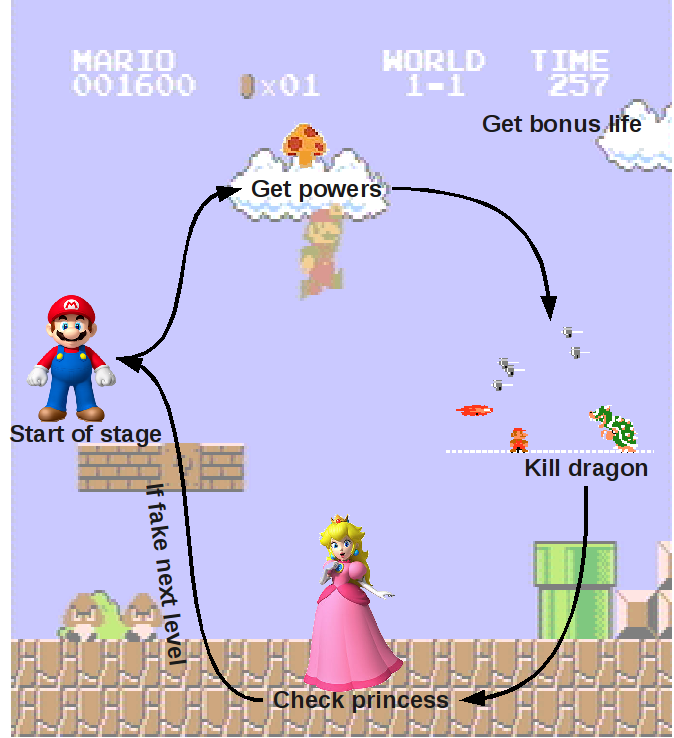
\includegraphics[height=2.5in,width=2.5in, interpolate=true]{mario}
  \end{center}  
  \emphbar{VCS provides power to save and resume from a stage.}
\end{frame}

\begin{frame}
  \frametitle{How is it done?}
  \begin{itemize}
  \item It keeps track of changes you make to a file. You can improvise, revisit, and amend.
  \item All procedure is logged/recorded, so you and others can follow the development cycle.
  \end{itemize}  
\end{frame}

\begin{frame}
  \frametitle{Do we really need this?}
  \emphbar{For team of people working remotely(even different computers/machines) on a project, use of version control is inevitable!}
  \vspace{0.15in}
  \emphbar{For single person: managing projects and assignments becomes easy}
  \vspace{0.15in}
  \pause
  \emphbar{\color{red}{It is a good habit!}}
\end{frame}

\begin{frame}
  \frametitle{Whats on the menu!}
  \begin{itemize}
  \item cvs (Concurrent Version System)
  \item svn (Subversion)
  \item hg (Mercurial)
  \item bzr (Bazaar)
  \item git
  \end{itemize}
  \inctime{10}
\end{frame}

% Introduction to jargon 
\section{Learning the Lingo!}

\begin{frame}
  \frametitle{Common jargon: Basic setup}
  \begin{itemize}
  \item Repository(repo):\\
        The folder with all files.
  \item Server:\\
        Machine with main inventory/repo.
  \item Client:\\
        Local machines with copy of main repo.
  \end{itemize}
\end{frame}

\begin{frame}
  \frametitle{Actions}
  \begin{itemize}
  \item Add:\\
    Adding file into the repo for the first time.
  \item Version:\\
    Version number(Die Hard 4.0).
  \item Head/Tip:\\
    Most recent revision/stage.
  \item Check out/Clone:\\
    Initial download of working copy.
  \item Commit:\\
    Saving(recording) a change.
  \item Change log/History:\\
    List of all past changes.
  \end{itemize}
\end{frame}

\begin{frame}
  \frametitle{Actions cont...}
  \begin{itemize}
  \item Branch:\\
    Separate local copy for bug fixing, testing.
  \item Diff/Change:\\
    Changes made in a file in two different versions.
  \item Merge (or patch):\\
    Appling the changes to file, to make it up-to-date.
  \item Conflict:\\
    When merging a file is not obvious.
  \item Resolve:\\
    Fixing the conflict manually.
  \end{itemize}
\end{frame}

% Types of Version Controls
\section{Types of VCS}

\begin{frame}
  \frametitle{Types:}
  Based on ways of managing the repo there are two types of VCS:
  \begin{itemize}
  \item Centralized VCS\\
    cvs, svn fall under this category.
  \item Distributed VCS\\
    hg, bzr, git follows this methodology.
  \end{itemize}
  \emphbar{We would be covering \typ{hg}}
\end{frame}

\begin{frame}
  \frametitle{Why hg?}
    
\includegraphics[height=.75in, interpolate=true]{mercurial}
  \begin{itemize}
  \item Easy to learn and use.
  \item Lightweight.
  \item Scales excellently.
  \item Written in Python.
  \end{itemize}
  \inctime{10}
\end{frame}

% Initializing the repo, cloning, committing changes, pushing, pulling to repo.
\section{Getting Started}

\begin{frame}[fragile]
  \frametitle{Getting comfortable:}
  For checking \typ{hg} installation and its version try:
  \begin{lstlisting}
    $ hg version    
  \end{lstlisting}
  To get broad help on \typ{hg} and commands available:
  \begin{lstlisting}
    $ man hg
    $ hg help
  \end{lstlisting}
  To get help on particular \typ{hg} related option try:
  \begin{lstlisting}
    $ hg help diff
  \end{lstlisting} %$
\end{frame}

\begin{frame}[fragile]
  \frametitle{Getting working/existing code base}
  \typ{clone} is used to make a copy of an existing repository. It can be both local or remote.
  \begin{lstlisting}
$ hg clone 
  http://hg.serpentine.com/tutorial/hello 
  localCopyhello
  \end{lstlisting}
  And we get a local copy of this repository. 
  \begin{lstlisting}
$ ls localCopyhello/
hello.c  Makefile
  \end{lstlisting}
\end{frame}

\begin{frame}[fragile]
  \frametitle{To start track-record on existing files}
  I have some files which I want to bring under version control. \typ{hg} provides \typ{init} command for this: 
  \begin{lstlisting}
$ ls -a circulate/
.  ..  lena.png  pendulum.txt  points.txt  pos.txt  sslc1.py  sslc1.txt
$ cd circulate/
$ hg init
$ ls -a
.  ..  .hg  lena.png  pendulum.txt  points.txt  pos.txt  sslc1.py  sslc1.txt    
  \end{lstlisting}
  \emphbar{\typ{.hg} directory keeps log of changes made henceforth.}
\end{frame}

\begin{frame}[fragile]
  \frametitle{Starting fresh}
  We can use \typ{init} to start a new repository also
  \begin{lstlisting}
$ mkdir Fevicol
$ cd Fevicol/
$ echo "print 'Yeh Fevicol ka majboot 
              jod hai'" > feviStick.py
$ ls -a
.  ..  feviStick.py
$ hg init
$ ls -a
.  ..  feviStick.py  .hg
  \end{lstlisting}
\end{frame}

\begin{frame}[fragile]
  \frametitle{Making copies: Branching}
  All \typ{hg} repositories are self-contained, and independent which can be copied(cloned):
  \begin{lstlisting}
$ hg clone localCopyhello newCopy
updating working directory
2 files updated, 0 files merged, 
0 files removed, 0 files unresolved
  \end{lstlisting}
  or
  \begin{lstlisting}
$ hg clone Fevicol Fevicol-pull
updating working directory
0 files updated, 0 files merged, 
0 files removed, 0 files unresolved
  \end{lstlisting}
  \inctime{20}
\end{frame}

%% Should we here stress on how are distribute VCS have 
%% different approach then centralized ones? Maybe a pic
%% or some other graphical representation.
\begin{frame}[fragile]
  \frametitle{Revisiting saved points:history/logs}
  In \typ{hg}, the difference between consecutive stages is termed as changeset.\\
  Once we have saved stages, we need a mechanism to review and access them, for that use \typ{log} command.
  \begin{lstlisting}
$ cd localCopyhello
$ hg log    
  \end{lstlisting}
\end{frame}

\begin{frame}[fragile]
  \frametitle{Understanding output}
  The output provides following information:
  \begin{itemize}
  \item changeset: Identifiers for the changeset.
  \item user: Person who created the changeset.
  \item date: Date and time of creation of changeset.
  \item summary: One line description.
  \end{itemize}
\end{frame}

\begin{frame}[fragile]
  \frametitle{History/Logs cont...}
  By default \typ{log} returns complete list of all changes. \\
  For selective view try:
\begin{lstlisting}
$ hg log -r 3
$ hg log -r 2:4
\end{lstlisting}
  tip/latest changes can be seen via:
  \begin{lstlisting}
$ hg tip    
  \end{lstlisting} %%$
  \inctime{5}
\end{frame}

\begin{frame}[fragile]
  \frametitle{Advancing through a stage:status}
  We often need to add/delete some files from directory(repo). The structure keeps on evolving, and tools for handling them are needed.\\
  We will use the Fevicol repo we created earlier.
  \begin{lstlisting}
$ cd Fevicol
$ hg log
$ hg st
? feviStick.py
  \end{lstlisting} %%$
  \typ{st} (aka status) is command to show changed files in the working directory.\\
\end{frame}

%% track record is confusing for some. Duma have some doubts :(
\begin{frame}[fragile]
  \frametitle{Adding files}
  "?" indicates that these file are aliens to track record.\\
  \typ{add} command is available to add new files to present structure.
  \begin{lstlisting}
$ hg add feviStick.py
$ hg st
A feviStick.py
  \end{lstlisting}
\end{frame}

\begin{frame}[fragile]
  \frametitle{Saving present stage: committing}
  \emphbar{This is equivalent to completing tasks, before reaching a stage where you want to save.}
  \typ{hg} uses \typ{ci}(aka \typ{commit}) command to save changes. So after adding file, we have to commit it also:
  \begin{lstlisting}
$ hg ci -u "Shantanu <shantanu@fossee.in>" 
        -m "First commit."
$ hg log
changeset:   0:84f5e91f4de1
tag:         tip
user:        Shantanu <shantanu@fossee.in>
date:        Fri Aug 21 23:37:13 2009 +0530
summary:     First commit.    
  \end{lstlisting}
\end{frame}

\begin{frame}[fragile]
  \frametitle{Other operations}
  \typ{hg} supports basic file-management functions like copy, remove, rename etc.
  \begin{lstlisting}
$ hg cp feviStick.py pidiLite.py
$ hg rename pidiLite.py feviCol.py
$ hg st
A feviCol.py
$ hg ci -u "Shantanu <shantanu@fossee.in>" 
        -m "Added feviCol.py."
$ hg tip| grep summary 
summary:     Added feviCol.py.
  \end{lstlisting} %$
%% Other commands which can be handy are \typ{remove}, \typ{revert} etc.
  \inctime{10}
\end{frame}

% Introduction to concepts of branches, merging patch?
\section{Sharing and Collaborating}

\begin{frame}[fragile]
  \frametitle{Distributing changes}
  \begin{itemize}
  \item All directory-structure(repo) are self-contained.
  \item Changes created are local.
    \begin{itemize}
    \item Until we sync. previously cloned repos.
    \end{itemize}
  \end{itemize}
  \begin{lstlisting}
$ hg pull 
pulling from /home/baali/Fevicol
requesting all changes
adding changesets
adding manifests
adding file changes
added 2 changesets with 2 changes to 2 files
(run 'hg update' to get a working copy)
  \end{lstlisting} %$
\end{frame}

\begin{frame}[fragile]
  \frametitle{Pulling changesets cont...}
  \typ{pull} command doesn't update current directory, it just imports changesets. To add all these changes, use \typ{up}:
  \begin{lstlisting}
$ cd Fevicol-pull
$ ls -a
.  ..  .hg
$ hg up
2 files updated, 0 files merged, 
0 files removed, 0 files unresolved
$ ls -a
.  ..  feviCol.py  feviStick.py  .hg    
  \end{lstlisting}
  \pause
  \emphbar{Why \typ{pull} and \typ{up} are needed separately?}
\end{frame}

\begin{frame}[fragile]
  \frametitle{Making changes across branches}
  \begin{lstlisting}
$ cd Fevicol-pull/
  \end{lstlisting} %$
  Lets edit and correct the feviStick.py 
\begin{lstlisting}
$ echo "print 'Ab no more Chip Chip'" 
        > feviStick.py
$ hg st
M feviStick.py
\end{lstlisting}
  'M' sign indicates that \typ{hg} has noticed change.\\
\end{frame}

\begin{frame}[fragile]
  \frametitle{Revisiting changes}
  To view changes made \typ{hg} provides \typ{diff}:
\begin{lstlisting}
$ hg diff
diff -r a7912d45f47c feviStick.py
--- a/feviStick.py   Sun Aug 23 22:34:35 2009 +0530
+++ b/feviStick.py   Sun Aug 23 22:47:49 2009 +0530
@@ -1,1 +1,1 @@
-print 'Yeh Fevicol ka Majboot jod hai'
+print 'Ab no more Chip Chip'
  \end{lstlisting} %$
\end{frame}

\begin{frame}[fragile]
  \frametitle{Saving the changes}
  We have to commit these changes.
  \begin{lstlisting}
$ hg ci -u "Shantanu <shantanu@fossee.in>" 
      -m "Changed tagline for feviStick.py."
  \end{lstlisting} %$
\end{frame}

\begin{frame}[fragile]
  \frametitle{Syncing two repos}
  To bring both the repos at same stage we have to \typ{push} differences.
  \begin{lstlisting}
$ hg push 
pushing to /home/baali/Fevicol
searching for changes
adding changesets
adding manifests
adding file changes
added 1 changesets with 1 changes to 1 files
  \end{lstlisting} %$
\end{frame}

\begin{frame}[fragile]
  \frametitle{Syncing cont...}
  Same as pulling, pushing wont update the main directory by default.
  \begin{lstlisting}
$ cd Fevicol
$ hg tip    
$ cat feviStick.py
  \end{lstlisting}
  \typ{tip} shows latest changeset, but content of file are not updated. We have to use \typ{up} on main branch
  \begin{lstlisting}
$ hg up
1 files updated, 0 files merged, 0 files removed, 0 files unresolved    
  \end{lstlisting} %$
  \inctime{15}
\end{frame}

\begin{frame}[fragile]
  \frametitle{Merging: Scenario}
  One very useful feature is merging work of different peers working on same project.\\
  We consider scenario, two person on one project, both have local copies, and one among them is main branch.\\
  \begin{center}
    
\includegraphics[height=1in, interpolate=true]{scenario}
  \end{center}  
\end{frame}

\begin{frame}[fragile]
  \frametitle{Making changes to one of repo}
  \begin{lstlisting}
$ cd Fevicol-pull
$ echo "print 'Yeh Fevicol ka Majboot jod 
        hai, tootega nahin'" > feviCol.py
$ hg st
M feviStick.py
$ hg ci -u "Shantanu <shantanu@fossee.in>" 
     -m "Updated tag line for feviCol.py."
$ hg tip| grep changeset
changeset:   3:caf986b15e05
  \end{lstlisting} %$
\end{frame}

\begin{frame}[fragile]
  \frametitle{In the meanwhile, other repo is ...}
  \begin{lstlisting}
$ cd Fevicol
$ echo "print 'Jor laga ke hayyiya'" 
        > firstAdd.py
$ hg add 
$ hg st
A firstAdd.py
$ hg ci -u "Shantanu <shantanu@fossee.in>"
        -m "Added firsAdd.py."
$ hg tip|grep changeset
changeset:   3:fadbd6492cc4    
  \end{lstlisting}
\end{frame}

%%\hspace*{-0.5in} 

\begin{frame}[fragile]
  \frametitle{Situation}
  \begin{columns}
    \column{0.5\textwidth}    
    \begin{block}{\center{main directory}}
      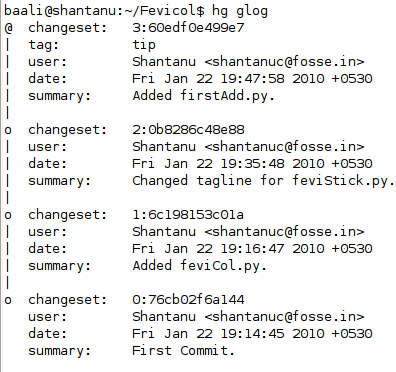
\includegraphics[height=2in, interpolate=true]{main}
    \end{block}
    \column{0.5\textwidth} 
    \begin{block}{\center{cloned directory}}
      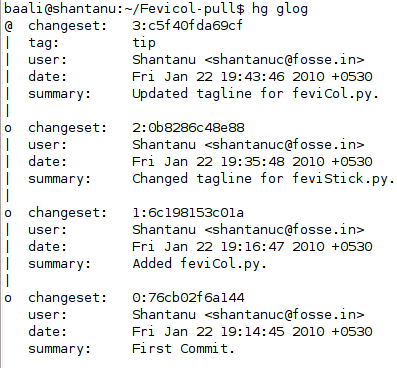
\includegraphics[height=2in, interpolate=true]{clone}
    \end{block}
  \end{columns}
\end{frame}

\begin{frame}[fragile]
  \frametitle{Merging}
  \begin{lstlisting}
$ hg pull ../Fevicol-pull
pulling from ../Fevicol-pull
searching for changes
adding changesets
adding manifests
adding file changes
added 1 changesets with 1 changes to 1 files (+1 heads)
(run 'hg heads' to see heads, 'hg merge' to merge)    
  \end{lstlisting} %$
  Output is already suggesting something!
\end{frame}

%% Here one can mention the point of having push and pull separate. Because of this policy, changes made are not lost.
\begin{frame}[fragile]
  \frametitle{Analyzing events in detail}
  Since hg \typ{pull} don't update the files directly, our changes are still safe. Following command can help us deal this merging problem in better way:
  \begin{lstlisting}
$ hg heads
  \end{lstlisting}
  This commands shows repo/branch heads.
  \begin{lstlisting}
$ hg glog    
  \end{lstlisting}
  It shows revision history alongside an ASCII revision graph.\\
  Because of different track, \typ{up} command fails.
  \begin{lstlisting}
$ hg up
abort: crosses branches (use 'hg merge' or 'hg update -C')
  \end{lstlisting} %$
\end{frame}

\begin{frame}[fragile]
  \frametitle{Merging}
  \typ{hg merge} command merge working directory with another revision.
  \begin{lstlisting}
$ hg merge    
  \end{lstlisting} %$
  After merging two branches, we have to commit the results to create a common head.
  \begin{lstlisting}
$ hg ci -u "Shantanu <shantanu@fossee.in>" 
        -m "Merged branches."
$ hg heads    
$ hg glog
  \end{lstlisting} %$
  \inctime{15}
\end{frame}

% Steps to follow to make life easier. How to avoid/handle manual merges.
\section{Work flow: DOS and DON'Ts}

\begin{frame}
  \frametitle{Motto behind hg}
  \begin{center}
  \color{red}{``Commit Early Commit Often.''}\\  
  \end{center}  
\end{frame}

\begin{frame}
  \frametitle{Cheat Sheet}
  \begin{center}
  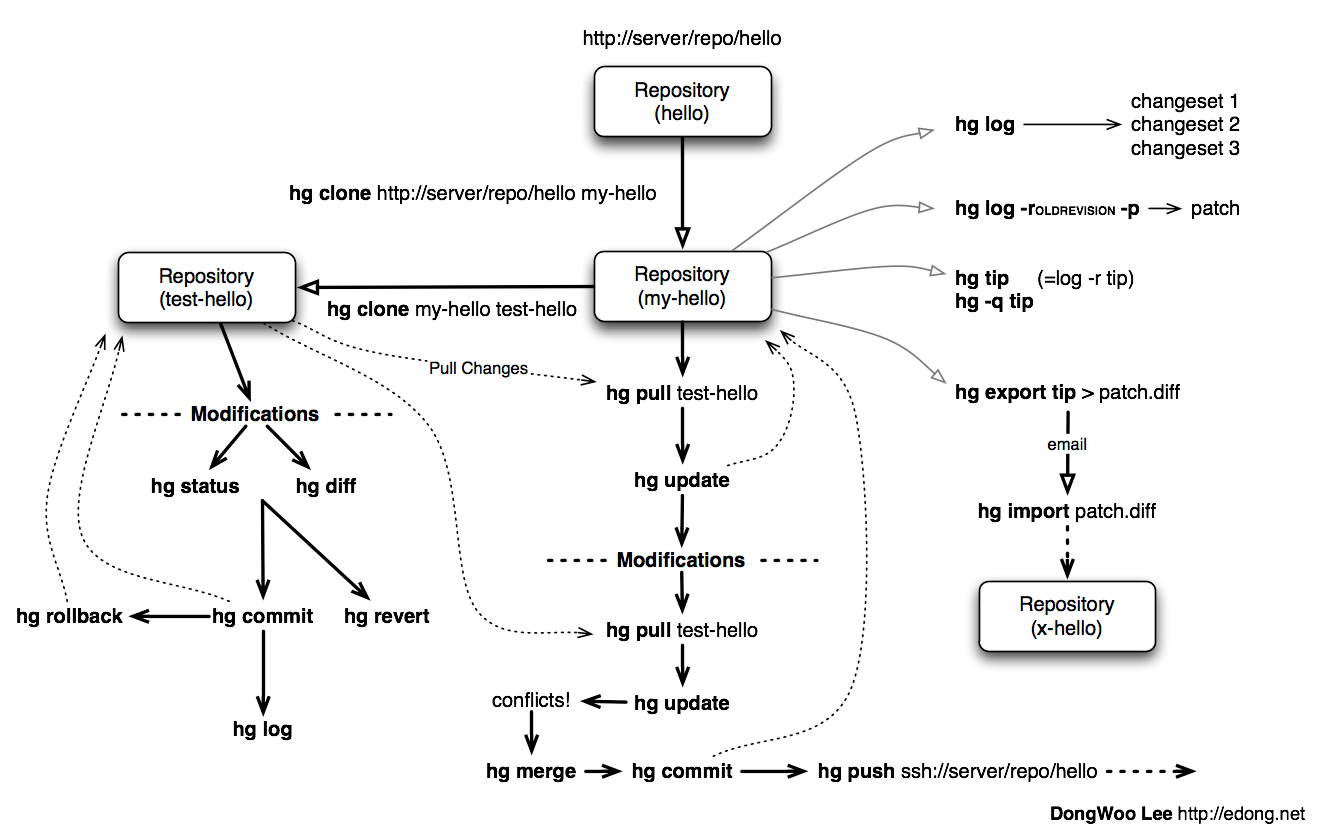
\includegraphics[height=2.8in]{mod}  
  \end{center}  
\end{frame}

\begin{frame}
  \frametitle{Steps to be followed}
  \begin{itemize}
  \item Make changes.
  \item Commit.
  \item Pull changesets.
  \item Merge(if required).
  \item Push.
  \end{itemize}
  \inctime{10}
\end{frame}

\begin{frame}
  \frametitle{Suggested Readings:}
  \begin{itemize}
  \item \url{http://mercurial.selenic.com/guide/}
  \item \url{http://hgbook.red-bean.com/}    
  \item \url{http://karlagius.com/2009/01/09/version-control-for-the-masses/}
  \item Articles related to version control available on \url{http://betterexplained.com/}
  \item \url{http://en.wikipedia.org/wiki/Revision_control}
  \item \url{http://wiki.alliedmods.net/Mercurial_Tutorial}
  \end{itemize}
\end{frame}
\end{document}

Notes
-----

From http://mercurial.selenic.com/

Quick Start

Clone a project and push changes

$ hg clone http://selenic.com/repo/hello
$ cd hello
$ (edit files)
$ hg add (new files)
$ hg commit -m 'My changes'
$ hg push


Create a project and commit

$ hg init (project-directory)
$ cd (project-directory)
$ (add some files)
$ hg add
$ hg commit -m 'Initial commit'
